\documentclass[12pt,a4paper]{article}

% packages.tex  (limpio, conserva tus paquetes originales)

% Custom vars
\def\gr{...}      % Set the group number cons. across doc
\def\nass{1}    % Set the assignment number cons. across doc
\def\cl{Econometrics }   % Define the class

% --------------------------
% Encoding & page geometry
% --------------------------
\usepackage[utf8]{inputenc}
\usepackage[T1]{fontenc}
\usepackage[
  a4paper,
  total={170mm,257mm},
  left=25mm,
  right=25mm,
  top=25mm,
  bottom=25mm
]{geometry}

% --------------------------
% Graphics, images, svg
% --------------------------
\usepackage{graphicx}
\usepackage{svg}                 
\graphicspath{{Latex/imgs/}}

% --------------------------
% Math, plots, tikz
% --------------------------
\usepackage{amsmath,amssymb}
\usepackage{mathtools}
\usepackage{pgfplots}
\pgfplotsset{width=12cm,compat=newest}
\usepackage{tikz}
\usetikzlibrary{shapes.geometric, arrows, positioning}

% --------------------------
% Figures, captions, tables
% --------------------------
\usepackage[font=small,labelfont=bf]{caption}
\usepackage{subcaption}          
\usepackage{booktabs}
\usepackage{makecell}
\usepackage{multirow}
\usepackage{threeparttable}
\usepackage{tabularx}
\usepackage{float}
\usepackage{wrapfig}
\usepackage{transparent}

% --------------------------
% Code highlighting (conservo ambos: minted y listings)
% --------------------------
% minted requiere --shell-escape al compilar (ver nota abajo).
\usepackage[newfloat]{minted}     % Code highlighting (más potente)
\newenvironment{code}{\captionsetup{type=listing}}{}
\SetupFloatingEnvironment{listing}{name=Code}

\usepackage{listings}            
\lstset{
  language=Python,
  basicstyle=\ttfamily\footnotesize,
  backgroundcolor=\color{gray!10},
  frame=single,
  keywordstyle=\color{blue},
  commentstyle=\color{green!50!black},
  stringstyle=\color{red!70!black}
}

\setminted{
    fontsize=\small,
    breaklines=true,
    linenos=true,
    autogobble=true,
    mathescape=true,
    breakanywhere=true,
    samepage=false
}

% --------------------------
% Utilities
% --------------------------
\usepackage{xcolor}
\usepackage{url}
\usepackage{enumitem}
\usepackage{xspace}
\usepackage{multicol}

% --------------------------
% Header / footer
% --------------------------
\usepackage{fancyhdr}
\fancyhf{}                           
\fancyhead[L]{DSDM - BSE}
\fancyhead[C]{\cl}
\fancyhead[R]{Assignment \nass}
\renewcommand{\headrulewidth}{0.4pt}
\fancyfoot[C]{\thepage}
\pagestyle{fancy}

% --------------------------
% Extras / includes / pdfpages
% --------------------------
\usepackage{pdfpages}
\usepackage{newclude}               % si usas \includeonly/\newinclude
\usepackage{csquotes}

% --------------------------
% Hyperref (una sola carga) + metadata
% --------------------------
\usepackage{hyperref}
\hypersetup{
    pdftitle    = {\cl - Assignment~\nass},
    pdfsubject  = {This is a submission in the DSDM Masters at BSE.},
    pdfauthor   = {Group~\gr},
    pdfcreator  = {Overleaf},
    pdfstartview= FitH
}

% --------------------------
% Bibliografía (biblatex)
% --------------------------
\usepackage[backend=biber, style=authoryear, hyperref=true]{biblatex}
\usepackage{csquotes}               
\DeclareCiteCommand{\cite}
  {\usebibmacro{prenote}}
  {\usebibmacro{citeindex}%
   \printnames{labelname}%
   \space(\printfield{year})}
  {\multicitedelim}
  {\usebibmacro{postnote}}
\DeclareNameAlias{labelname}{family-given}
\renewcommand*{\nameyeardelim}{\addcomma\space}
\AtEveryCitekey{\ifciteseen{}{\defcounter{maxnames}{1}}}
\addbibresource{Latex/chapters/references.bib}

% --------------------------
% Espaciado / estilo de párrafo
% --------------------------
\setlength{\parskip}{0.3\baselineskip}
\setlength{\parindent}{0pt}
\linespread{1.15}

% --------------------------
% List of code (adecuado para article -> uso section)
% --------------------------
\renewcommand{\listoflistings}{
  \cleardoublepage
  \addcontentsline{toc}{section}{List of Code} 
  \listof{listing}{List of Code}
}


\usepackage{fancyhdr}
\setlength{\headheight}{15pt}  % Increase header height
\addtolength{\topmargin}{-3pt}  % Adjust top margin to compensate

\begin{document}

% Title page
\begin{titlepage}
\centering

\includegraphics[width=0.75\textwidth]{LaTex/imgs/bse_logo.pdf}
\par\vspace{0.75cm}
	{\huge\bfseries Assignment 4 \par}
    {\large\bfseries Foundations of Econometrics \\
                        Group 7\par}
	\vspace{0.25cm}
    \noindent\rule{\textwidth}{1pt}
    {\Large 
        \par}
    \noindent\rule{\textwidth}{1pt}
	\vfill
	{\large \today\par}
\end{titlepage}
\newpage

\section*{Question 1}
Class slide 3(33) (Unit 3) illustrated, via simulation, the effects of collinearity. The script used to generate the sample is included in file \texttt{data33.R}.

\subsection*{Part (a)}
\begin{enumerate}[label=(\roman*)]
  \item Estimate the regression model included in the slide, presenting OLS estimates and the 95\% confidence intervals for each parameter; Include the output in your answer.
  
  \textbf{Answer:} 
 
\begin{table}[ht]
    \centering
    \caption{Regression Results with 95\% CI} 
    \label{tab:regression}
  \begin{tabular}{rrrrr}
    \hline
    & Estimate & Std..Error & Lower & Upper \\ 
    \hline
    (Intercept) & 7.9365 & 1.6426 & 4.5863 & 11.2867 \\ 
    x2 & 0.5953 & 0.0747 & 0.4429 & 0.7476 \\ 
    x3 & 0.2996 & 0.5264 & -0.7740 & 1.3733 \\ 
    x4 & 0.7818 & 0.5277 & -0.2945 & 1.8582 \\ 
    \hline
  \end{tabular}
\end{table}

  
  \item Using \texttt{confidenceEllipse()} function, or equivalent, draw the 95\% confidence region for parameters $\beta_3$, $\beta_4$. Include also in the drawing the confidence intervals for each parameter.
  
  \textbf{Answer:} 

    \begin{figure}[H]  % Capital H forces it exactly here
      \centering
      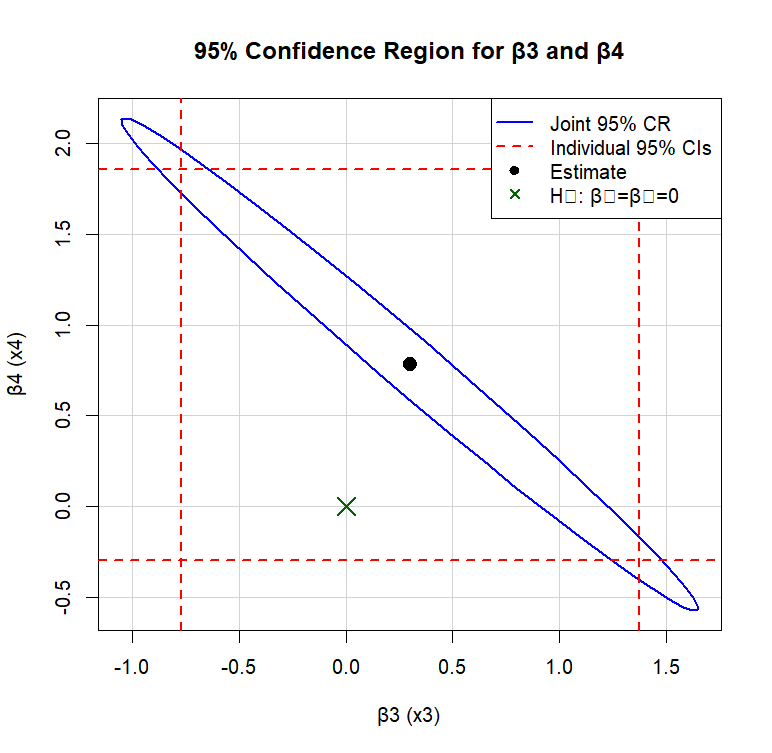
\includegraphics[width=0.5\textwidth]{Files/q1ii_plot.png}
      \caption{95\% Confidence Region for $\beta_3$ and $\beta_4$}
      \label{fig:ellipse}
    \end{figure}

  \item Describe what the confidence region you just drew provides.
  
  \textbf{Answer:} 

  The confidence region we drew illustrates the joint confiendence region, while the red lines show the individual confidence intervals.
  It represents every combination of the two parameters that falls in the 95\% confidence region. It also illsutrates the
  correlation between the two parameters, as the confidence region is elongated along a diagonal line. The negative slope provides 
  insight into the negative correlation between the two parameters.
  
  \item Use the figure of confidence intervals and confidence region to show the difference between testing statistical significance of regressors separately or jointly, and explain why this is so relevant under the presence of collinear regressors.
  
  \textbf{Answer:} 

The figure illustrates that joint testing can show us when collinear variables are jointly significant,
even if they are not individually significant.

\textbf{Individual tests:} Testing $H_0: \beta_3=0$ and 
$H_0: \beta_4=0$ separately uses the rectangular region formed by the 
individual 95\% confidence intervals (red dashed lines). From the regression output,
both intervals include zero: $x_3$ CI 
$= [-0.7740, 1.3733]$ and $x_4$ CI $= [-0.2945, 1.8582]$. Since the 
rectangle contains the origin $(0,0)$, we fail to reject both null 
hypotheses individually---neither $x_3$ nor $x_4$ appears statistically 
significant.

\textbf{Joint test:} Testing $H_0: \beta_3=\beta_4=0$ jointly uses the 
95\% confidence ellipse. The ellipse is much smaller than the rectangle 
due to the negative correlation between $\hat{\beta}_3$ and 
$\hat{\beta}_4$. If the origin $(0,0)$ falls outside the ellipse, we 
reject the joint null hypothesis, meaning $x_3$ and $x_4$ are jointly 
significant even though neither is individually significant.

\textbf{Collinearity:} When regressors are collinear, their 
coefficients are negatively correlated because if one increases, the other
must decrease to fit the same 
data. This creates the tilted ellipse. The individual tests ignore this 
correlation and use the wider rectangular region, making them overly 
conservative. The joint test correctly accounts for correlation, 
revealing that while we cannot precisely determine which variable drives 
the effect, we can confidently say that together they have a significant 
impact on $y$. This demonstrates why collinearity makes individual 
$t$-tests unreliable while joint $F$-tests remain valid.


\end{enumerate}

\subsection*{Part (b)}
Modify the script used to estimate now the same regression with data generated from the same dgp but now using a sample of 3500 observations.

\begin{enumerate}[label=(\roman*)]
  \item Surprised with how the estimates have changed? Rigorously justify.

  \textbf{Answer:} 

latex\subsection*{Part (b)}
Modify the script used to estimate now the same regression with data 
generated from the same dgp but now using a sample of 3500 observations.

\begin{enumerate}[label=(\roman*)]
  \item Surprised with how the estimates have changed? Rigorously justify.
  
  \textbf{Answer:} 
  
  Not surprised. The estimates have converged closer to the true parameter 
  values ($\beta_3=\beta_4=0.5$, shown by purple dotted lines in Figure 
  \ref{fig:comparison}). For $n=35$, the estimates were $\hat{\beta}_3=0.2996$ 
  and $\hat{\beta}_4=0.7818$, showing considerable sampling variability. 
  With $n=3500$, the estimates are much closer to 0.5 for both parameters.
  
  By the Law of Large Numbers, as sample size increases, the OLS estimators 
  converge in probability to their true values. This is consistency: 
  $\text{plim}(\hat{\beta}_j) = \beta_j$ as $n \to \infty$. The larger 
  sample provides more information about the true relationship, reducing 
  the influence of random sampling variation. The collinearity between $x_3$ 
  and $x_4$ still exists (since $x_4 = x_3 + \text{noise}$ in both samples), 
  but with more observations, the estimator can better distinguish their 
  individual effects on $y$.
  
  
  \item Surprised of the change of the 95\% confidence intervals? Rigorously justify.
  
  \textbf{Answer:} 
  
  \item Surprised of the change of the 95\% confidence region for parameters $\beta_3$, $\beta_4$? Rigorously justify.
  
  \textbf{Answer:} 
  
  \item Using the variance decomposition expression for $\text{var}(\hat{\beta}_3 \mid X)$, or $\text{var}(\hat{\beta}_4 \mid X)$, discuss why increasing $n$ can explain the changes observed. Be specific.
  
  \textbf{Answer:} 
\end{enumerate}

\subsection*{Part (c)}
Now, go back to the original script generating 35 observations, and modify the script so that now $x_{i3} + 2x_{i4} = 0$.

\begin{enumerate}[label=(\roman*)]
  \item Run the script again. Include the output in your answer.
  
  \textbf{Answer:} 
  
  \item How many estimates did you get an estimate for $\beta_3$? And for $\beta_4$? You should be able to show, using the proper derivation, that in fact you got an infinite number of estimates for $\beta_3$ and $\beta_4$.
  
  \textbf{Answer:} 
\end{enumerate}

\newpage

\section*{Question 2}
Data file \texttt{microsoft.csv} includes monthly data from May 1986 to April 2013 on $RP_{msft}$ (excess return of Microsoft stock), $RP_{s\&p}$ (excess return on the S\&P500 portfolio), $Dprod$ (variation of Industrial production), $Dinflation$ (change in inflation rate), $Dterm$ (change in interest rate) and $m1$ (an indicator variable that takes value 1 if $t$ is the month of January and 0 otherwise). The following regression is set to measure the reaction of the excess return of Microsoft stocks to changes in macroeconomic variables:
\[
RP_{msft,t} = \beta_1 + \beta_2 RP_{s\&p,t} + \beta_3 Dprod_t + \beta_4 Dinflation_t + \beta_5 Dterm_t + \beta_6 m1_t + \epsilon_t
\]

\begin{enumerate}[label=(\alph*)]
  \item Estimate the model above by OLS. Present the complete output (estimates, standard errors, p-values) as your answer.
  
  \textbf{Answer:} 

  \begin{center}
\begin{tabular}{lclc}
\toprule
\textbf{Dep. Variable:}    &     RPmsoft      & \textbf{  R-squared:         } &     0.213   \\
\textbf{Model:}            &       OLS        & \textbf{  Adj. R-squared:    } &     0.201   \\
\textbf{Method:}           &  Least Squares   & \textbf{  F-statistic:       } &     17.26   \\
\textbf{Date:}             & Wed, 22 Oct 2025 & \textbf{  Prob (F-statistic):} &  4.08e-15   \\
\textbf{Time:}             &     12:54:20     & \textbf{  Log-Likelihood:    } &   -1276.7   \\
\textbf{No. Observations:} &         324      & \textbf{  AIC:               } &     2565.   \\
\textbf{Df Residuals:}     &         318      & \textbf{  BIC:               } &     2588.   \\
\textbf{Df Model:}         &           5      & \textbf{                     } &             \\
\textbf{Covariance Type:}  &    nonrobust     & \textbf{                     } &             \\
\bottomrule
\end{tabular}
\begin{tabular}{lcccccc}
                    & \textbf{coef} & \textbf{std err} & \textbf{t} & \textbf{P$> |$t$|$} & \textbf{[0.025} & \textbf{0.975]}  \\
\midrule
\textbf{const}      &      -0.9291  &        0.760     &    -1.223  &         0.222        &       -2.424    &        0.566     \\
\textbf{RPsandp}    &       1.3232  &        0.152     &     8.678  &         0.000        &        1.023    &        1.623     \\
\textbf{Dprod}      &      -1.5216  &        1.283     &    -1.186  &         0.237        &       -4.046    &        1.003     \\
\textbf{Dinflation} &       0.4716  &        2.351     &     0.201  &         0.841        &       -4.154    &        5.097     \\
\textbf{Dterm}      &       4.1587  &        2.487     &     1.672  &         0.095        &       -0.735    &        9.052     \\
\textbf{m1}         &       5.4352  &        2.869     &     1.894  &         0.059        &       -0.210    &       11.081     \\
\bottomrule
\end{tabular}
\begin{tabular}{lclc}
\textbf{Omnibus:}       & 203.965 & \textbf{  Durbin-Watson:     } &    2.141  \\
\textbf{Prob(Omnibus):} &   0.000 & \textbf{  Jarque-Bera (JB):  } & 1809.211  \\
\textbf{Skew:}          &  -2.541 & \textbf{  Prob(JB):          } &     0.00  \\
\textbf{Kurtosis:}      &  13.401 & \textbf{  Cond. No.          } &     21.2  \\
\bottomrule
\end{tabular}
%\caption{OLS Regression Results}
\end{center}

Notes: \newline
 [1] Standard Errors assume that the covariance matrix of the errors is correctly specified.
  
  \item The January effect states that on average, every else equal, the returns (or excess returns) are larger in the month of January than the rest of the months. Test, at $\alpha = 1\%$, the presence of the January effect using the exact $t$-test statistic. Would you say the data supports the presence of this effect?
  
  \textbf{Answer:} 

  We test for the presence of the January effect by examining whether the coefficient on the January dummy variable ($m_1$) is statistically significant.

  \textbf{Hypotheses:}
  \begin{align*}
      H_0: \beta_6 &= 0 \quad \text{(No January effect)} \\
      H_1: \beta_6 &\neq 0 \quad \text{(January effect exists)}
  \end{align*}

  We use a two-tailed $t$-test at significance level $\alpha = 0.01$.

    \textbf{Test Statistic:}
      \[
          t = \frac{\hat{\beta}_6}{\text{SE}(\hat{\beta}_6)} = \frac{5.44}{2.87} = 1.89
      \]

  With 318 degrees of freedom, the critical values are $\pm 2.59$. So, reject $H_0$ if $|t| > 2.59$ or equivalently if $p < 0.01$.
  The $t$-statistic is 1.89 with a $p$-value of 0.059. Since $|1.89| < 2.59$ and $p = 0.059 > 0.01$, we fail to reject the null hypothesis.
  Therefore, we do not have sufficient evidence at the 1\% significance level to conclude that there is a January effect in Microsoft stock returns.
  
  \item Aside from normality, list the assumptions needed to justify the use of the $t$ test statistic. Justify your answer.
  
  \textbf{Answer:} 
  
  \item For the test you performed in questions (2b), you were asked to use the $t$ test statistic. Using this test requires, among others, for disturbances to be normally distributed. One of the available tests of normality of the distribution of a given random variable is the Jarque-Bera test. Under the null hypothesis of normality, the Jarque-Bera (JB) test statistic is:
  \[
  JB \equiv \frac{n}{6}\left[sk^2 + \frac{(kur - 3)^2}{4}\right] \stackrel{a}{\sim} \chi^2(2),
  \]
  where $sk$ is the sample coefficient of skewness of the variable and $kur$ is its sample coefficient of kurtosis. Using a significance level of 1\%, draw (by hand absolutely fine) the distribution of JB under $H_0$ and the corresponding acceptance and rejection regions. Provide an intuition for the location of the acceptance region.
  
  \textbf{Answer:} 
  
  \item Now, we want to test for the presence of normality in our disturbances using the JB test. Ideally, to test normality of disturbances, JB test should be applied to a sample of disturbances, but, given that they are unobservable, the JB test is usually applied to our OLS residuals. Explain how, if all the assumptions regarding the dgp for consistency of OLS estimator are met, it would be justified for $\hat{\epsilon}_t$'s to take the place of $\epsilon_t$'s to perform the test.
  
  \textbf{Answer:} 
  
  \item Perform the JB test on the OLS residuals. What do you conclude? Comment.
  
  \textbf{Answer:} 
  
  \item Repeat the test performed in (2b) using the asymptotic $T$-test statistic. Use a 1\% significance level.
  
  \textbf{Answer:} 
  
  \item Is the use of asymptotic tests justified in this case? Rigorously argue.
  
  \textbf{Answer:} 
  
  \item Consider the following statement: ``Using the exact $t$ test statistic leads to slightly more conservative inference, because we get larger acceptance regions and larger $p$-values than if we used the asymptotic version.'' Do you agree? Rigorously argue.
  
  \textbf{Answer:} 
\end{enumerate}

\end{document}